\chapter{Местность на плане 1752 года}

\begin{center}
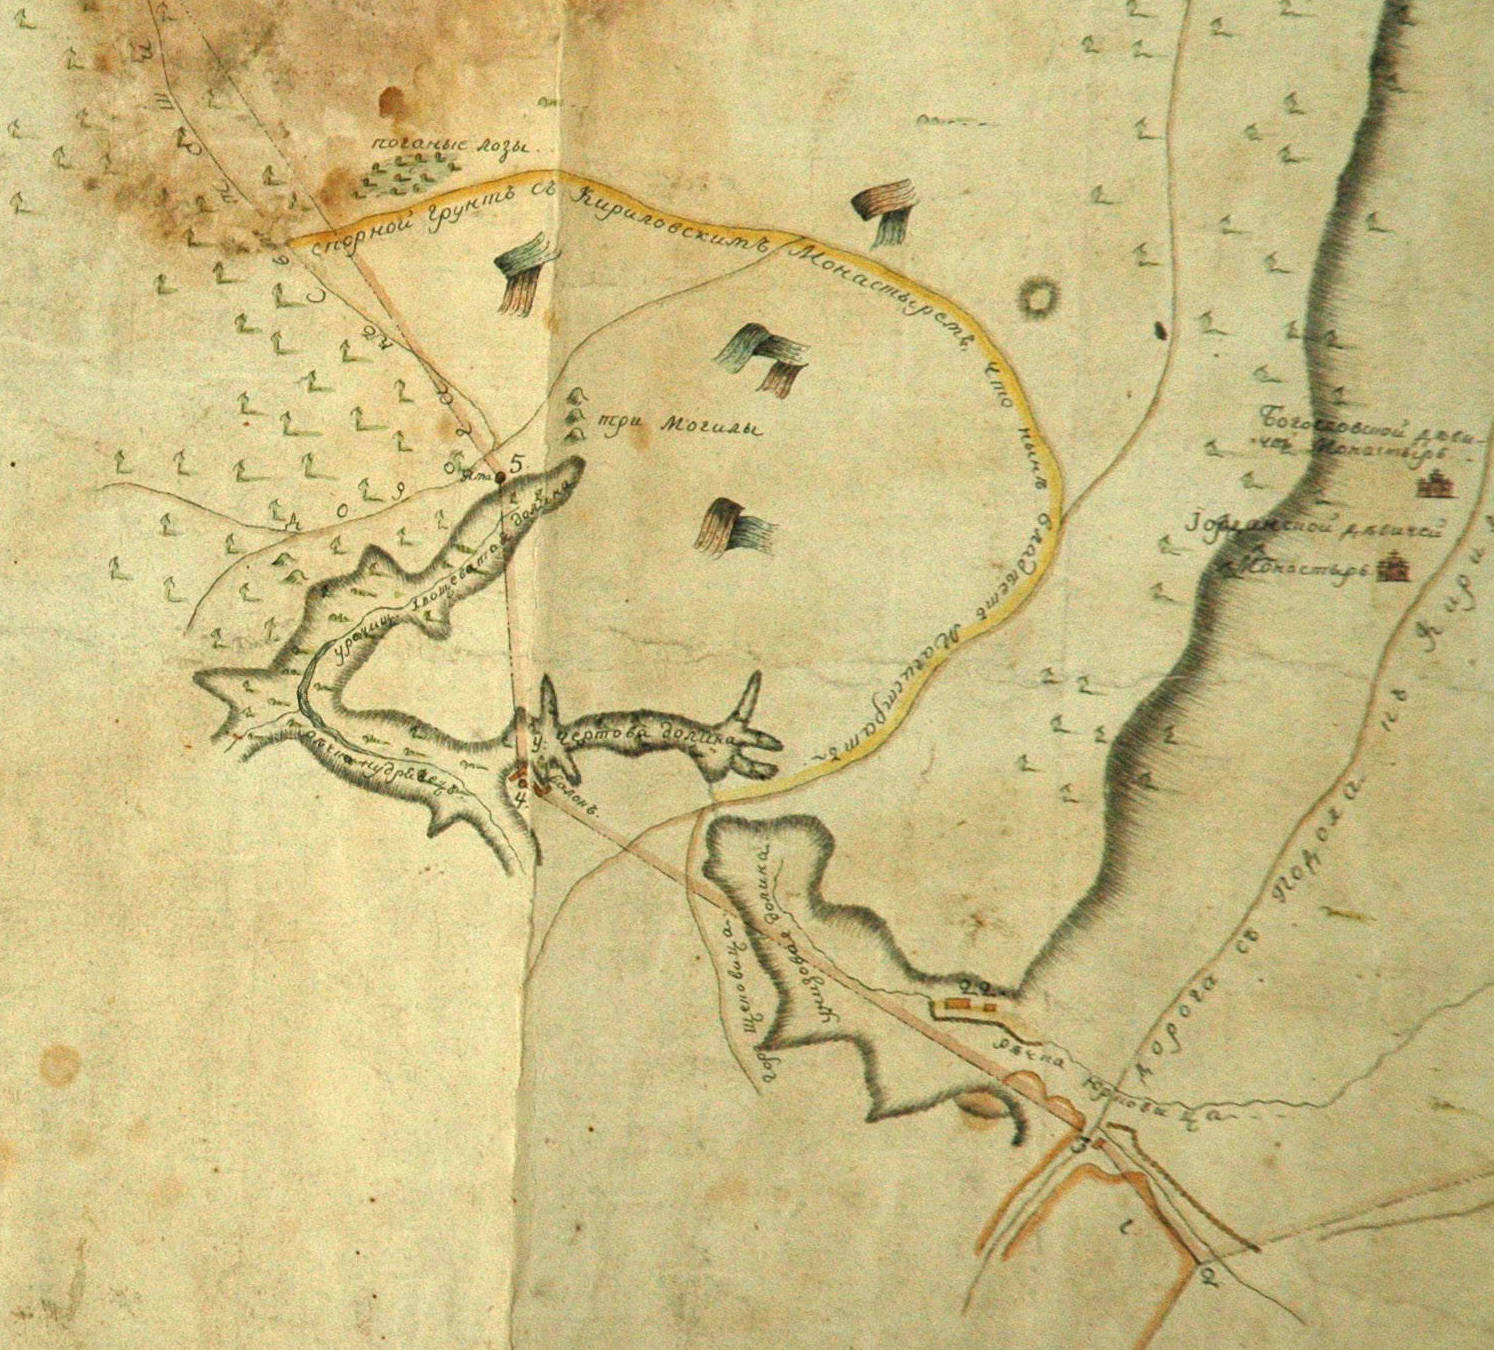
\includegraphics[width=\linewidth]{chast-kirvys/1752/1752y.jpg}
\end{center}

Полностью «Карта снятая и свидетельствованная по Дукту дьяка Алферова спорных земель по иску Киево-Кирилловского монастыря с Киевским Магистратом» приведена в главе про Почайну, здесь же мы разберем ее кусок, относящийся к Кирилловским высотам и окрестностям.

Сперва сопровождающее карту описание, где помимо словесных, по пунктам, описаний урочищ – точек границы – указано сколько саженей от одной точки к другой, хотя при утере множества упомянутых ориентиров и при том, что не пишется в какую сторону отсчитывать эти сажени, многое остается неясным. Весь текст легенды карты, не только по рассматриваемому нами куску, таков:

\begin{quotation}
НАДПИСЬ НУМЕРАМ

1. Строение, часть города Нижнего Киева называемаго Подола

2. От старожитнаго валка до Иорданских\footnote{В подлиннике «Їорданскихъ».} рогаток по показанию сторожилов промеж дорогою что лежит с Подолу к Кириловскому Монастырю копаны были столбы и поставлены кресты мерою 135 сажней.

3. От Иорданских рогаток через гору Щекавицу и Чертову долину до валка что у Кудрявца над буераком мерою 570 сажней.

4. От валка чрез буерак же Кудрявцем и Хвощеватою долиною на дорогу, что ездят из Киева к Светошицкому бору, а до ямы --- мерою 270 сажней.

5. От ямы тоюж дорогою до урочища Данилова Креста и Поганых лоз и до ямы мерою 1010 сажней.

6. От ямы и до урочища Данилова Креста тоюж дорогою до вершины речки Сырца а до ямы мерою 1300 сажней.

7. От вершины речки Сырца вниз речкою до верхней Кириловской мелницы мерою 1500 сажней.

8. От Кириловской верхней мелницы до Пещаного взвоза где переезжают речку Сырец мерою 68 сажней.

9. От дороги и Пещаного взвоза вниз речкою Сырцем до урочища Пунищ мерою 1400 сажней.

10. От Пунищ Речищем до урочища Круговины что на излучине, и до ямы мерою 570 сажней.

11. От Круговины до Долгого Кириловского озера где оной Сырец напред течение имел мерою 350 сажней.

12. От устья Сырца тем же Кириловским озером до Иорданского озера и до ямы где сошлись Кривая и другая почаная и до ямы мерою 1145 сажней.

13. В верх же тем озером Долгим что лежит дорога к Выш-городу у смуговины, и до ямы мерою 275 сажней.

14. От ямы ж по Смуговине и до ямы --- мерою 475 сажней.

15. От ямы ж до другой ямы, где напред сего Крестное хождение было, мерою 200 сажней.

16. От ямы чрез Михайловское озеро против Сырца середнею дорогою, и до ямы мерою 400 сажней.

17. От ямы ж оной против (слово неразборчиво, может «песков») к долгому озеру мерою 550 сажней.

18. От ямы по Турцу и смуговине мерою 485 сажней.

19. От смуговины ж до старожитнаго вала мерою 485 сажней.

20. Речка Сырец где ныне свое течение имеет от нумера 21-го, от того места оной Сырец по показанию Сторожилов разлылся по ровным местам болота. 

22. Кирпичные заводы Мещанина Ивана Григоровича, который речку Юрковицу принял на одну сажень ---

Красною тушевною значит что ныне свидетельствовано по дукту дьяка Алферьева а желтою тушевною значит спорное, что Киевский Магистрат ныне владеет внутрь Алфериева дукту.

Копировал Киевскаго Главнаго Народнаго Училища ученик Наум Рыбачков. 1794 20 августа.

(неразборчово, затем) учитель Иван Карбан???кий
\end{quotation}

Напомню, карта ориентирована так, что север находится справа. Относительно разбираемой нами местности примечательно следующее.

Показаны Иорданский и Богословский девичьи монастыри. «Речка Юрковица» и кирпичный завод Ивана Григоровича на самом юго-восточном углу Лысой горы (современной Юрковицы).

Речка Кудрявец, вытекающая из Хвощеватой долины. Чуть выше поворота Кудрявца, слева, на берегу видны два кургана. Еще три кургана изображены вертикальным рядом у начала оврага Хвощеватой долины, и подписаны «Три могилы». Почти оттуда же отходит дорога на Святошицкий бор. 

Где искать все эти курганы, особенно три в ряд? Последние можно примерно поместить в местность за яром с истоком Кудрявца-Глубочицы, эдак у перекрестка Багговутовской и Овручской. Конечно, там всё застроено, однако побродить по задворкам улиц Герцена, Пугачёва, даже Мельникова не помешает. А быть может бывшая у перекрестка церковь святого Феодора стоит на земле прежних курганов, как знать?

Запомним на будущее, что где-то близ устья Глубо\-чицы-Кудрявца были три кургана, да еще два ниже по руслу. Курганная однако местность.
